\chapter{Referencial Teórico}
\label{cap:ref-teorico}
Neste capítulo serão apresentados os fundamentos pertinentes a este trabalho. A Seção \ref{ref-teo:npm} apresenta o conceito e o funcionamento do \gls{NPM} bem como a questão das dependências. A Seção \ref{ref-teo:prov_clie} distingue os termos \textit{provedor} e \textit{cliente}. Também para diferenciar termos, a Seção \ref{ref-teo:pac_rel_ver} conceitua as palavras \textit{pacote}, \textit{release} e \textit{versão}.

A Seção \ref{ref-teo:breaking_change} define o conceito de \textit{Breaking Change}.

\section{\gls{NPM}}
\label{ref-teo:npm}
O \gls{NPM} é um gerenciador de pacotes para o \textit{Node.js}. Lançado em 2009, seu principal objetivo é facilitar o compartilhamento de códigos escritos em \textit{Javascript}. Atualmente, o \gls{NPM} ocupa a posição de maior repositório para uma dada linguagem, com mais de 1 milhão de projetos\footnote{http://www.modulecounts.com/}. O \gls{NPM} permite que, com apenas um simples comando, o usuário realize o download, publique, instale e desinstale pacotes diretamente do repositório. A facilidade proporcionada pelo \gls{NPM} corrobora para a grande popularidade do \textit{Javascript} e para que o compartilhamento de biblioteca seja largamente utilizado, uma vez que 97\% dos aplicativos \textit{web} são oriundos do \textit{NPM}\footnote{https://blog.npmjs.org/post/180868064080/this-year-in-javascript-2018-in-review-and-npms}.

O ecossistema \gls{NPM} estimula o compartilhamento de código entre aos pacotes. Por causa disso, o \gls{NPM}, dentre os demais repositórios, contém a maior distribuição de dependência entre os pacotes \cite{teorical_reference:npm_2}. Desta maneira, como muitos pacotes estão dependendo mutuamente uns dos outros, há uma gigantesca rede de interconectividade entre os pacotes. Entretanto, quando há um erro qualquer em algum destes pacotes, um grande número de outros pacotes podem ser afetados. Foi exatamente isso que ocorreu com um pacote chamado \textit{left-pad}\footnote{https://blog.npmjs.org/post/141577284765/kik-left-pad-and-npm}. Este pacote foi removido do \textit{NPM} por seu desenvolvedor e impactou milhares de pacotes em apenas 2.5 horas incluindo pacotes renomados como o \textit{babel}\footnote{https://github.com/babel/babel} e o \textit{atom}\footnote{https://github.com/atom/atom} que, devido ao grande número de dependentes, cascatearam o erro para inúmeros outros pacotes.
%In fact, 97\% of the code in a modern web application comes from npm

\section{Provedor e Cliente}
\label{ref-teo:prov_clie}
O pacote provedor é aquele que provê recursos ao pacote cliente, ou seja, contém interfaces públicas para acesso às suas funcionalidades. O termo \textit{pacote provedor} pode ser interpretado como \textit{bibliotecas} ou \textit{dependências}. É do provedor que emana a responsabilidade de indicar o nível de compatibilidade que sua nova \textit{release} está introduzindo \cite{teorical_reference:semver}. Por exemplo, quando é executado o seguinte comando

\begin{lstlisting}[style=bash, label=cod:install:provider]
npm install any_package
\end{lstlisting}
o \gls{NPM} salva o \textit{any\_package} no \textit{package.json} como uma dependência. Nesse momento, o \textit{any\_package} se torna um pacote provedor. Assim, o pacote \textit{any\_package} é um provedor direto, pois foi instalado diretamente pelo usuário. Entretanto, as dependências do \textit{any\_package} também são instaladas, mas de forma indireta pelo \gls{NPM}. Estes outros pacotes são chamados de \textit{provedores indiretos}, pois não dependem que o usuário instale-os diretamente com o comando \textit{npm install}.

Já o pacote cliente é aquele que está acessando as interfaces públicas do provedor. Quando uma \textit{break change} é introduzida pelo provedor -- direto ou indireto --, é sempre no pacote cliente que esta \textit{break change} se manifesta, causando o encerramento da execução. O pacote cliente é aquele que possui a responsabilidade de atualizar a versão de seus provedores no \textit{package.json} quando esses publicam uma \textit{release} com correções.

\section{Pacote, \textit{Release} e Versão}
\label{ref-teo:pac_rel_ver}
Neste artigo, a palavra \textit{pacote} refere-se a um \textit{software} hospedado no \gls{NPM}. Este \textit{software} contém seu nome, seus arquivos e suas versões. Por exemplo, quando nos referimos ao pacote \textit{mocha}, nos referimos à ideia genérica deste pacote, sem levar em consideração uma versão específica ou seu estado em algum instante, mas sim, apenas ao pacote como um todo.

Já a palavra \textit{release} designa o estado de um pacote em um determinado instante. uma \textit{release} é denotada por uma versão específica deste pacote, isto é, um conjunto de arquivos distintos das demais \textit{releases}. Cada \textit{release} é acompanhada da publicação de uma nova versão do pacote no \gls{NPM}.

Por fim, o termo \textit{versão} é utilizado para especificar e distinguir um determinado estado de uma \textit{release}. Uma \textit{versão} é uma \textit{string} no padrão \gls{SemVer} que identifica unicamente uma determinada \textit{release} e é utilizada pelo \gls{NPM} no arquivo \textit{package.json} para especificar um \textit{range} de versões que o cliente aceita.

\section{Node.js}
\label{ref-teo:node}
O \textit{Node.js} é um projeto \textit{open-source} implementado em \textit{C++} sobre a \textit{engine Javascript V8} do \textit{Google}, que é um compilador \textit{Javascript} para \textit{web}. O \textit{Node.js} foi criado com o objetivo de estender o código \textit{Javascript} para além do \textit{front-end} de forma que o \textit{Javascript} possa ser executado no \textit{back-end} também. Com o \textit{Javascript} executando no \textit{front-end} e no \textit{back-end} não se faz necessário que os desenvolvedores saibam duas linguagens de programação diferentes. A utilização do \textit{Javascript} no \textit{front} e no \textit{back-end}, através do \textit{Node.js}, foi um dos principais fatores que levou à grande popularidade do \textit{Javascript}, uma vez que o \textit{Node.js} é o \textit{framework} mais utilizado atualmente, de acordo com o \textit{Stack Overflow}\footnote{https://insights.stackoverflow.com/survey/2019\#technology-\_-other-frameworks-libraries-and-tools}.

\section{\gls{SemVer}}
\label{ref-teo:semver}
O \gls{SemVer}\footnote{https://semver.org} é um padrão para versionamento de \textit{releases} de um projeto a partir do tipo de alteração introduzida na \textit{release}. Com o \gls{SemVer} é possível evoluir um projeto sempre mantendo a compatibilidade com versões anteriores através de um \textit{range de versões} na qual está especificada uma determinada versão. O padrão \gls{SemVer} é largamente utilizada no desenvolvimento de projetos. As regras do \gls{SemVer} foram idealizadas por Tom Preston-Werner -- criador do \textit{GitHub} -- que incentiva todos os desenvolvedores à utilizarem este padrão, uma vez que as regras são baseadas em práticas comuns já utilizadas em projetos \cite{teorical_reference:semver}.

O esquema de versionamento, basicamente, é uma \textit{string} que possui três dígitos: \textit{major.minor.path}. Os dígitos do \gls{SemVer} devem ser incrementados de acordo com o tipo de alteração que a \textit{release} do projeto está introduzindo. O número \textit{major} deve ser incrementado quando uma \textit{release} introduz \textit{breaking changes}; o \textit{minor}, quando é adicionada melhorias/novas funcionalidades que mantenham a compatibilidade com as \textit{releases} anteriores; e o \textit{path}, quando a \textit{release} contém correção de \textit{bugs}. Com a padronização do \gls{SemVer} é possível que os desenvolvedores introduzem \textit{breaking changes} sem que essas afetem os clientes, uma vez que, por meio da \textit{string} de versionamento, eles não receberão a \textit{release} com \textit{breaking changes}.

O \gls{NPM} utiliza o padrão \gls{SemVer} no arquivo \textit{package.json} -- arquivo de configuração do projeto que contém todas as suas dependências e suas respectivas versões. Ao executar o comando \textit{npm install express --save}, para instalar a dependência \textit{express}\footnote{https://www.npmjs.com/package/express} por exemplo, o \gls{NPM} -- além de descarregar essa dependência -- irá salvar no \textit{package.json} o nome dessa dependência com sua versão atual em modo \textit{range}, de acordo com a Figura \ref{fig:dep_express}.

\begin{figure}
    \centering
    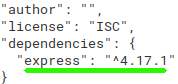
\includegraphics{figuras/dependencies_express.png}
    \caption{Modo como o \gls{NPM} salva no \textit{package.json} a versão de uma dependência}
    \label{fig:dep_express}
\end{figure}{}

Com a informação da versão da dependência no \textit{package.json}, o cliente não precisa se preocupar com as novas atualizações de sua dependência, uma vez que o \gls{NPM}, ao instalar novamente as dependências, sempre irá descarregar a \textit{release} mais recente da dependência que não contenha uma \textit{breaking change}, ou seja, a última \textit{release} disponível para a mesma versão \textit{major} -- desde que a \textit{string} de versionamento seja salva em modo \textit{range} (\textasciicircum).

\section{Breaking Change}
\label{ref-teo:breaking_change}
Uma \textit{break change} é uma alteração no pacote provedor que resulta em erros inesperados nos pacotes clientes, uma vez que versões prévias do pacote provedor executava normalmente \cite{teorical_reference:semver}. O conceito de \textit{breaking changes} não se refere exclusivamente à \textit{erros} causados pelos provedores, mas sim à mudanças nos pacotes. Durante o desenvolvimento de \textit{software}, esses precisam introduzir \textit{breaking changes}, pois quando só há \textit{releases} compatíveis com versões anteriores o pacote perde muitas oportunidades de evolução \cite{teorical_reference:bc_2}. Entretanto, a \textit{breaking change} pode ser introduzida em uma \textit{release} intencionalmente -- quando é atualizada a versão \textit{major} da \textit{release} --, mas também pode ser introduzida impremeditadamente -- quando é atualizada sua versão no \textit{minor} ou \textit{path} da \textit{release}. Sempre que \textit{breaking changes} são introduzidas inesperadamente, há grandes chances de ocorrer falhas no código cliente.

As \textit{breaking changes} são mais expressivas em linguagem fortemente tipadas, tais como \textit{.NET} e \textit{Java}, tanto que há ferramentas para detectar \textit{breaking changes} nestas linguagens. Já nas linguagens dinâmicas, como a linguagem \textit{Javascript}, as \textit{breaking changes} surgem com menos frequências e nem possuem ferramentas para detectar as \textit{breaking changes} \cite{teorical_reference:bc_1}. Como exemplo da dinâmica da linguagem \textit{Javascript}, considere a Figura \ref{fig:non-bc-async}.

\begin{figure}
    \centering
    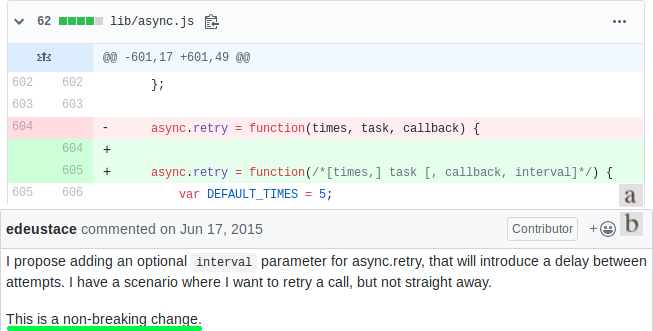
\includegraphics[scale=0.6]{figuras/non-bc-async.png}
    \caption{(a) alteração \textit{non-breaking change} entre duas \textit{releases minor}; (b) comentário do desenvolvedor afirmando que sua alteração não é uma \textit{breaking change}}
    \label{fig:non-bc-async}
\end{figure}{}

Na Figura \ref{fig:non-bc-async} (a) há uma alteração em uma das \gls{API} do pacote \textit{async} entre as \textit{releases 1.2.1-1.3}. Nesta alteração, houve a remoção da lista de parâmetros da função \textit{async.retry}. Em uma linguagem tipada, como o \textit{Java}, a alteração da lista de parâmetros é uma \textit{breaking change} e foi constatado como a terceira maior causa de \textit{breaking changes} em bibliotecas hospedados no \textit{Maven} -- repositório de bibliotecas em \textit{Java} -- em um estudo realizado por \citeonline{teorical_reference:semver}.

Entretanto, em linguagens dinâmicas como a linguagem \textit{Javascript}, a alteração da lista de parâmetros não é considerada uma \textit{breaking change}, pois o desenvolvedor que realizou o \textit{pull-request}\footnote{https://github.com/caolan/async/pull/793} da \ref{fig:non-bc-async} (a) comentou que esta alteração não é uma \textit{breaking change}, conforme a da Figura \ref{fig:non-bc-async} (b). Realmente, não é uma \textit{breaking change}, uma vez que uma chamada para a função \textit{async.retry}, seja na \textit{release 1.2.1} ou na \textit{release 1.3}, o código executa normalmente. Mesmo com esta alteração, um código irá executar em qualquer versão, uma vez que o \textit{node.js} insere os argumentos da chamada de função em um \textit{Array}, o que permite que qualquer função possa ser executada com qualquer número de argumentos\footnote{https://developer.mozilla.org/en-US/docs/Web/JavaScript/Reference/Functions/arguments}. Mesmo com a dinâmica da linguagem \textit{Javascript}, essa possui sim \textit{breaking changes}.